\chapter{Beispiele}
Im Folgenden wird eine beispielhafte Interaktion eines Nutzers mit dem System anhand von Bildschirmabzügen erläutert. In diesem Szenario will der fiktive Nutzer eine Buchung für Zimmer in dem Grandline-Hotel tätigen. Im ersten Schritt besucht der Nutzer die Startseite und klickt auf den \glqq buchen\grqq-Knopf (siehe Abb.\ref{step1}).
\begin{figure}
	\includegraphics[width=\textwidth]{images/Beispiel/Schritt1.png}
	\caption{Schritt 1}
	\label{step1}
\end{figure}
\newline
Als Folge des Klicks auf den \glqq buchen\grqq-Knopf kommt ein Formular (siehe Abb.\ref{step2}) hervor in welchem der Nutzer die Reisedaten und Anzahl der Zimmer für die gewünschte Buchung angeben kann.
\begin{figure}
	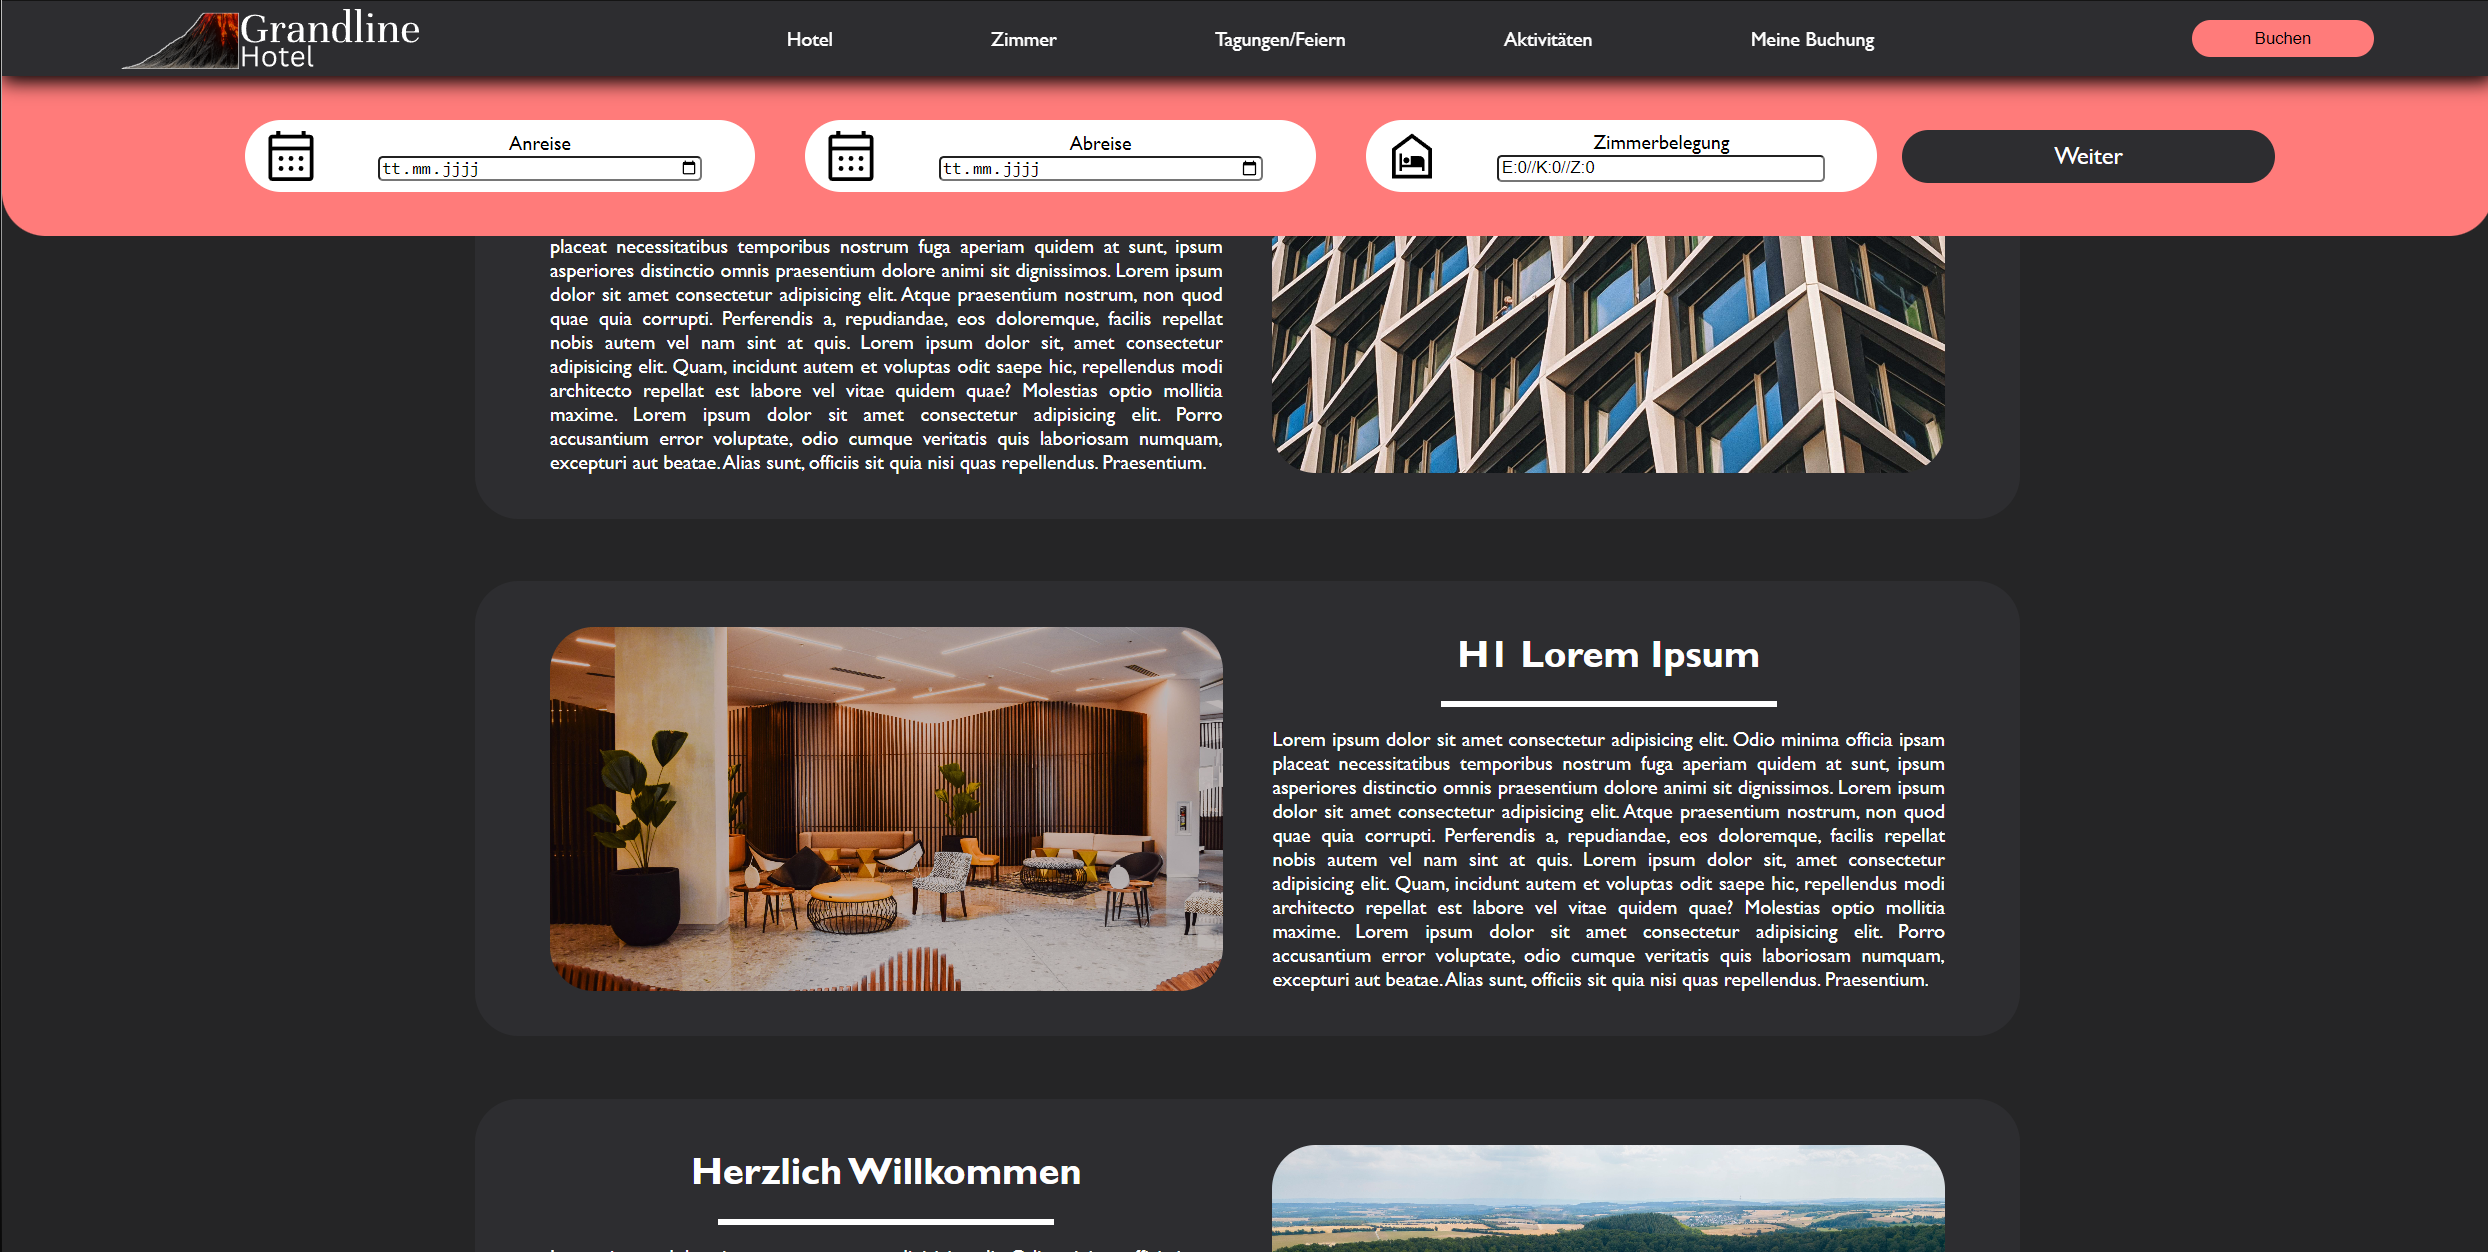
\includegraphics[width=\textwidth]{images/Beispiel/Schritt2.png}
	\caption{Schritt 2}
	\label{step2}
\end{figure}
\newpage In dem 3.Schritt tätigt der Nutzer seine Angaben in das Formular und setzt durch einen Klick auf den \glqq weiter\grqq-Knopf mit der Buchung fort (siehe Abb.\ref{step3}).
\begin{figure}
	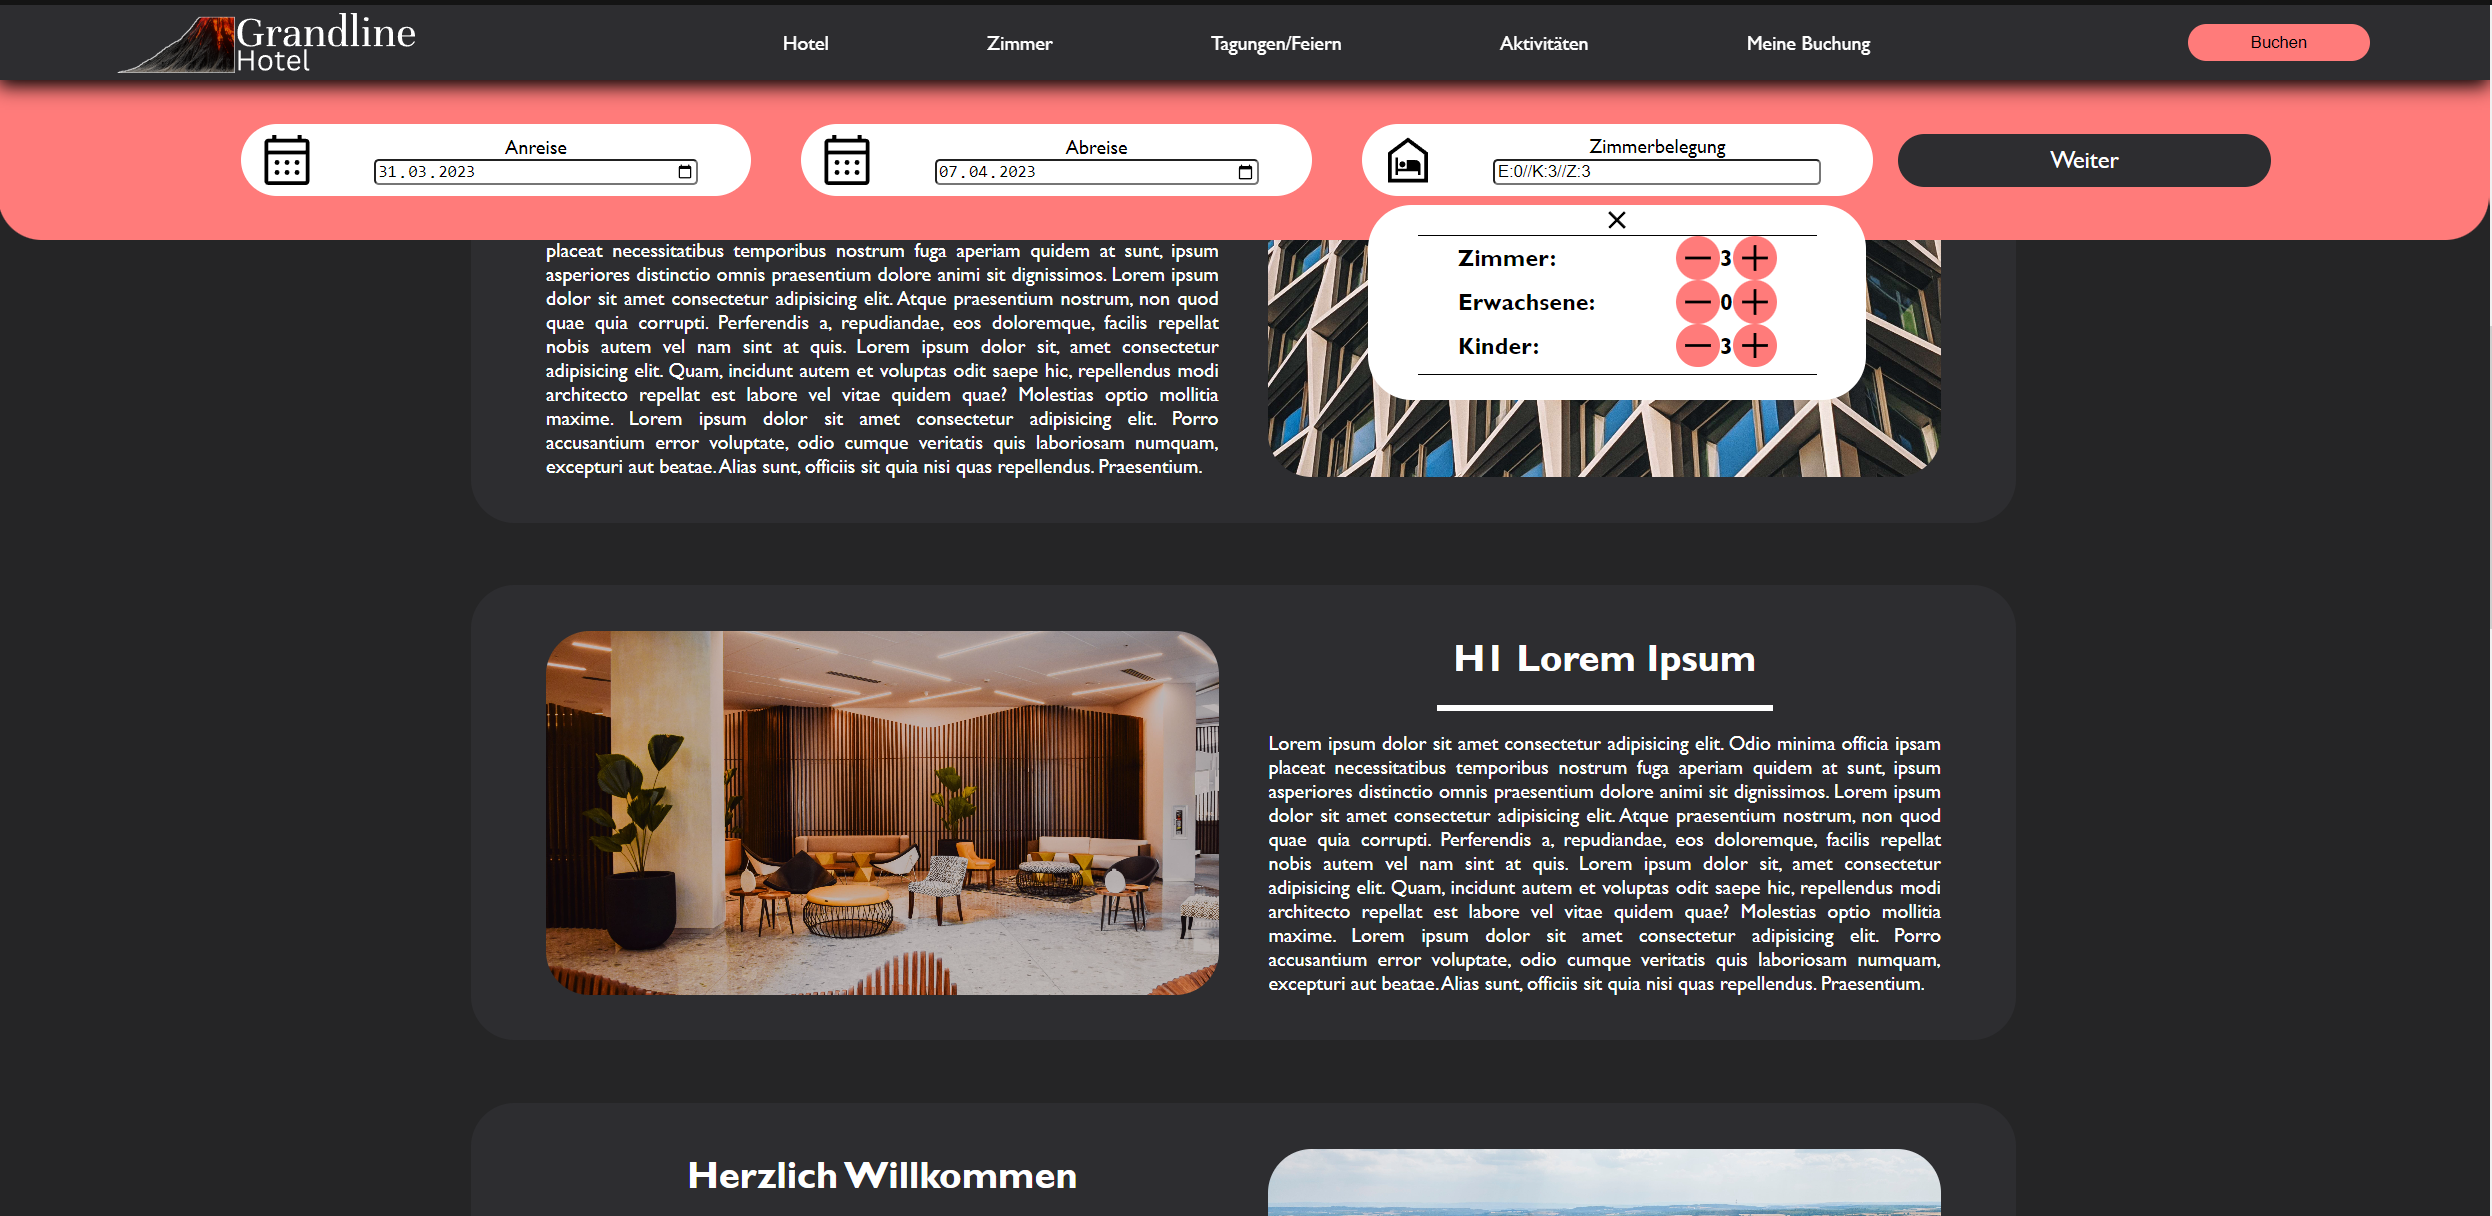
\includegraphics[width=\textwidth]{images/Beispiel/Schritt3.png}
	\caption{Schritt 3}
	\label{step3}
\end{figure}
\newline
Der Nutzer wird nun in den Buchungsdialog weitergeleitet in dem er eine Auswahl der verfügbaren Zimmer dargeboten bekommt (siehe Abb.\ref{step4}).
\begin{figure}
	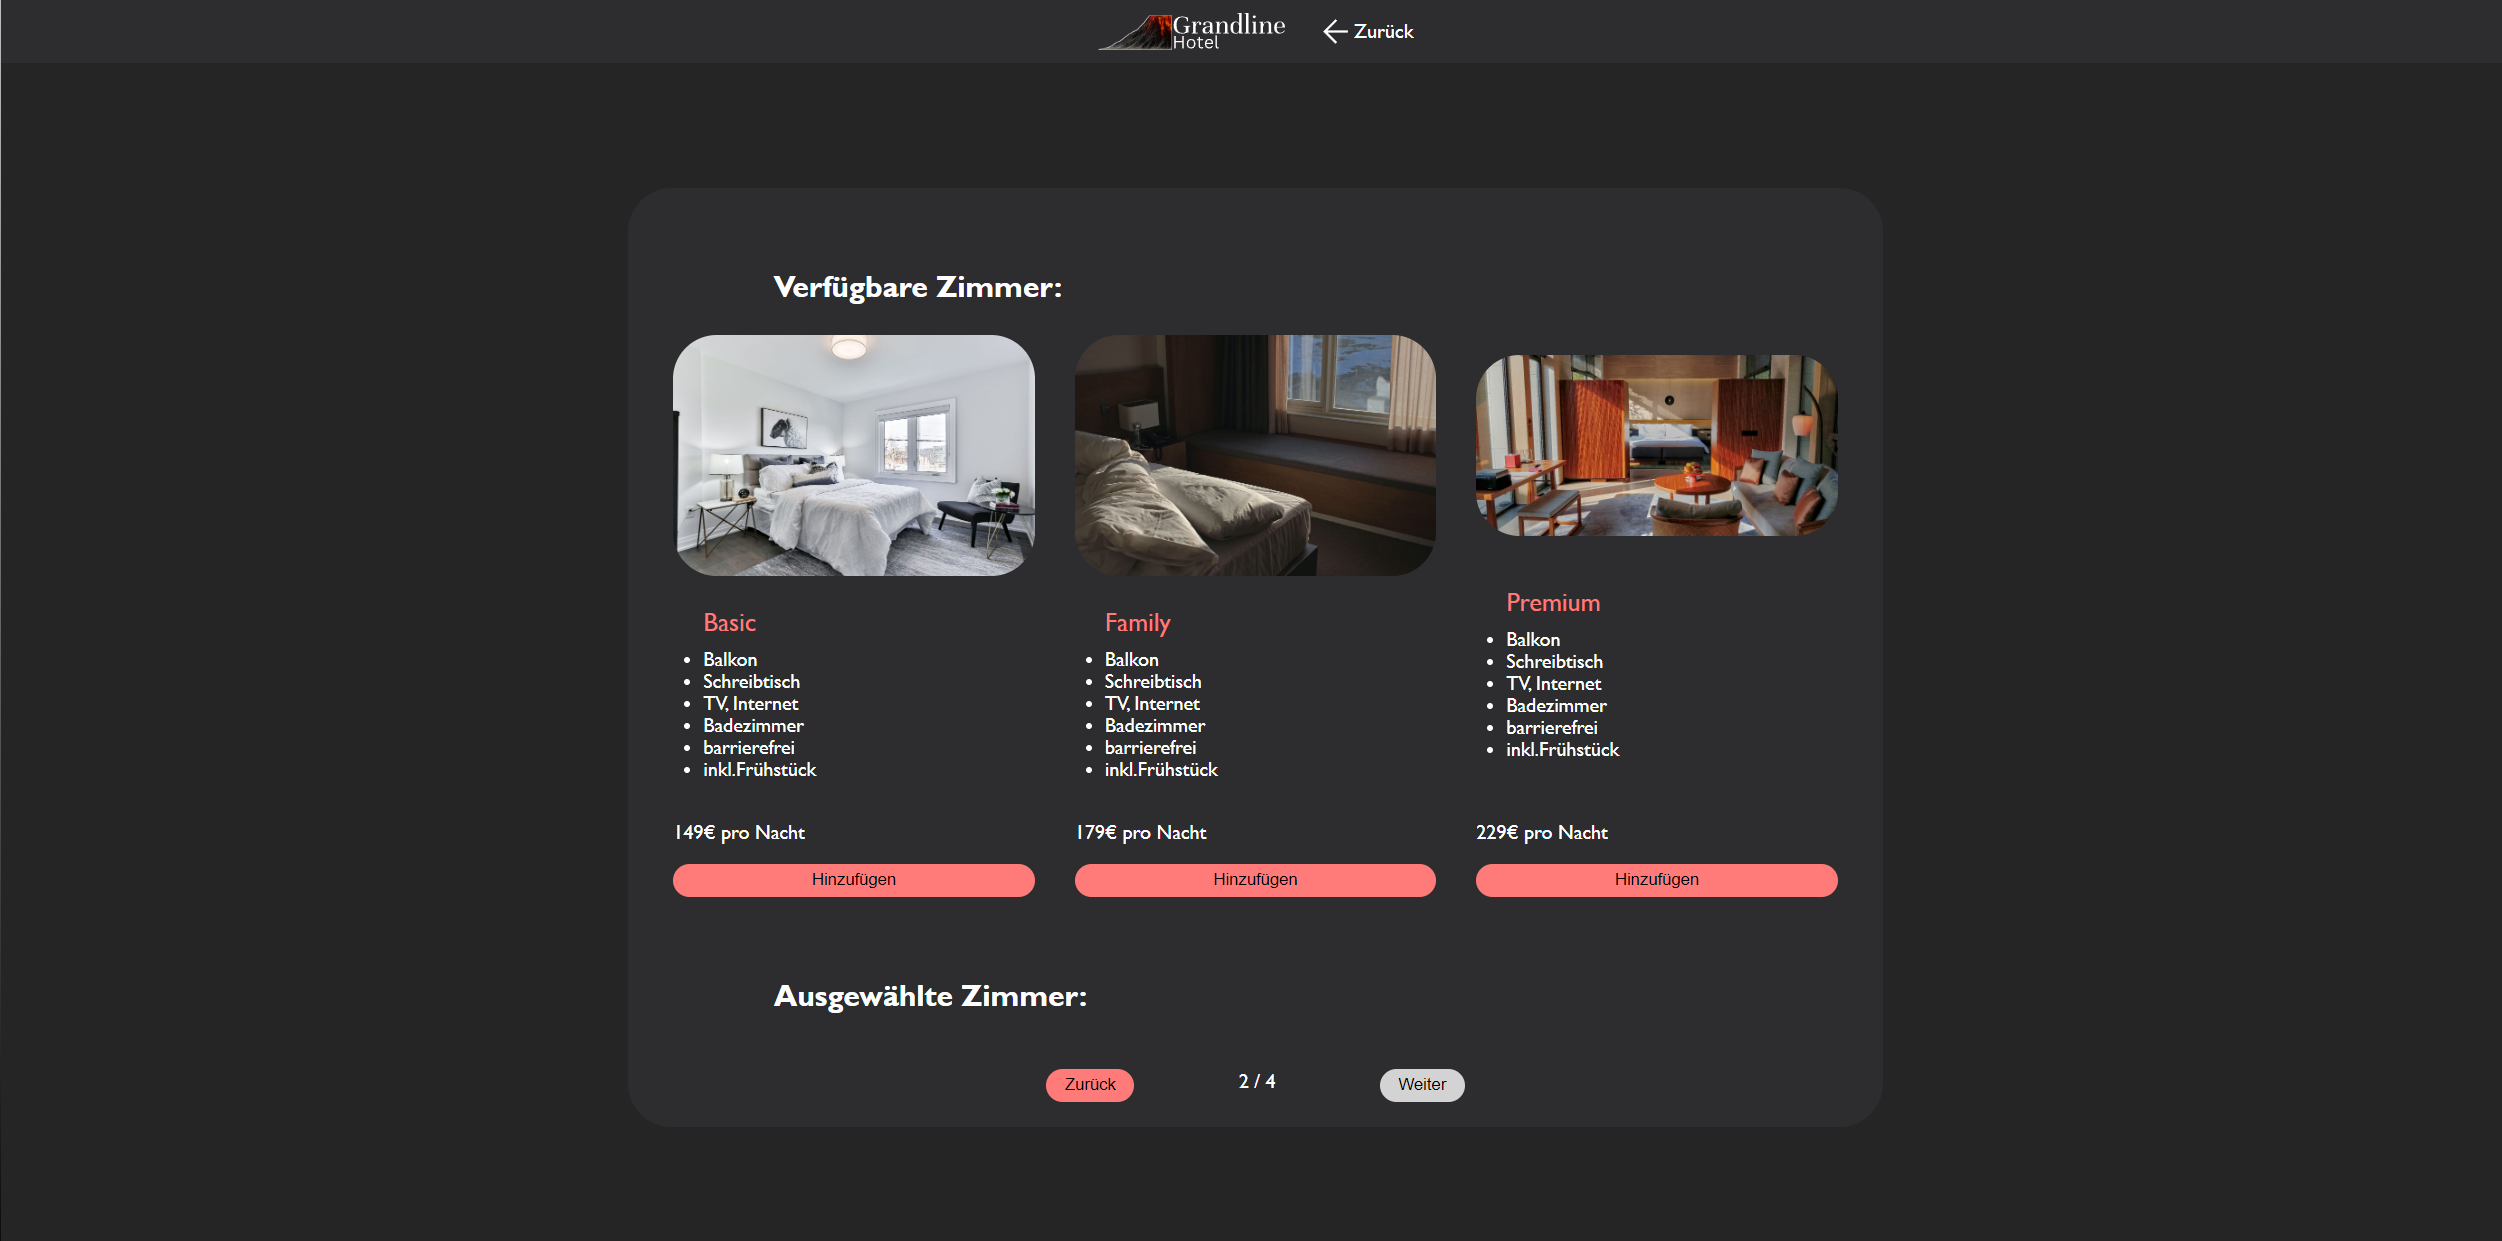
\includegraphics[width=\textwidth]{images/Beispiel/Schritt4.png}
	\caption{Schritt 4}
	\label{step4}
\end{figure}
\newpage
Der Nutzer wählt im 5. Schritt aus den verfügbaren Zimmern die Gewünschten aus und betätigt die \glqq Weiter\grqq-Taste (siehe Abb.\ref{step5}). Die Menge die der Nutzer auswählen muss entspricht der angegebenen Anzahl der Zimmer aus Schritt 3.
\begin{figure}
	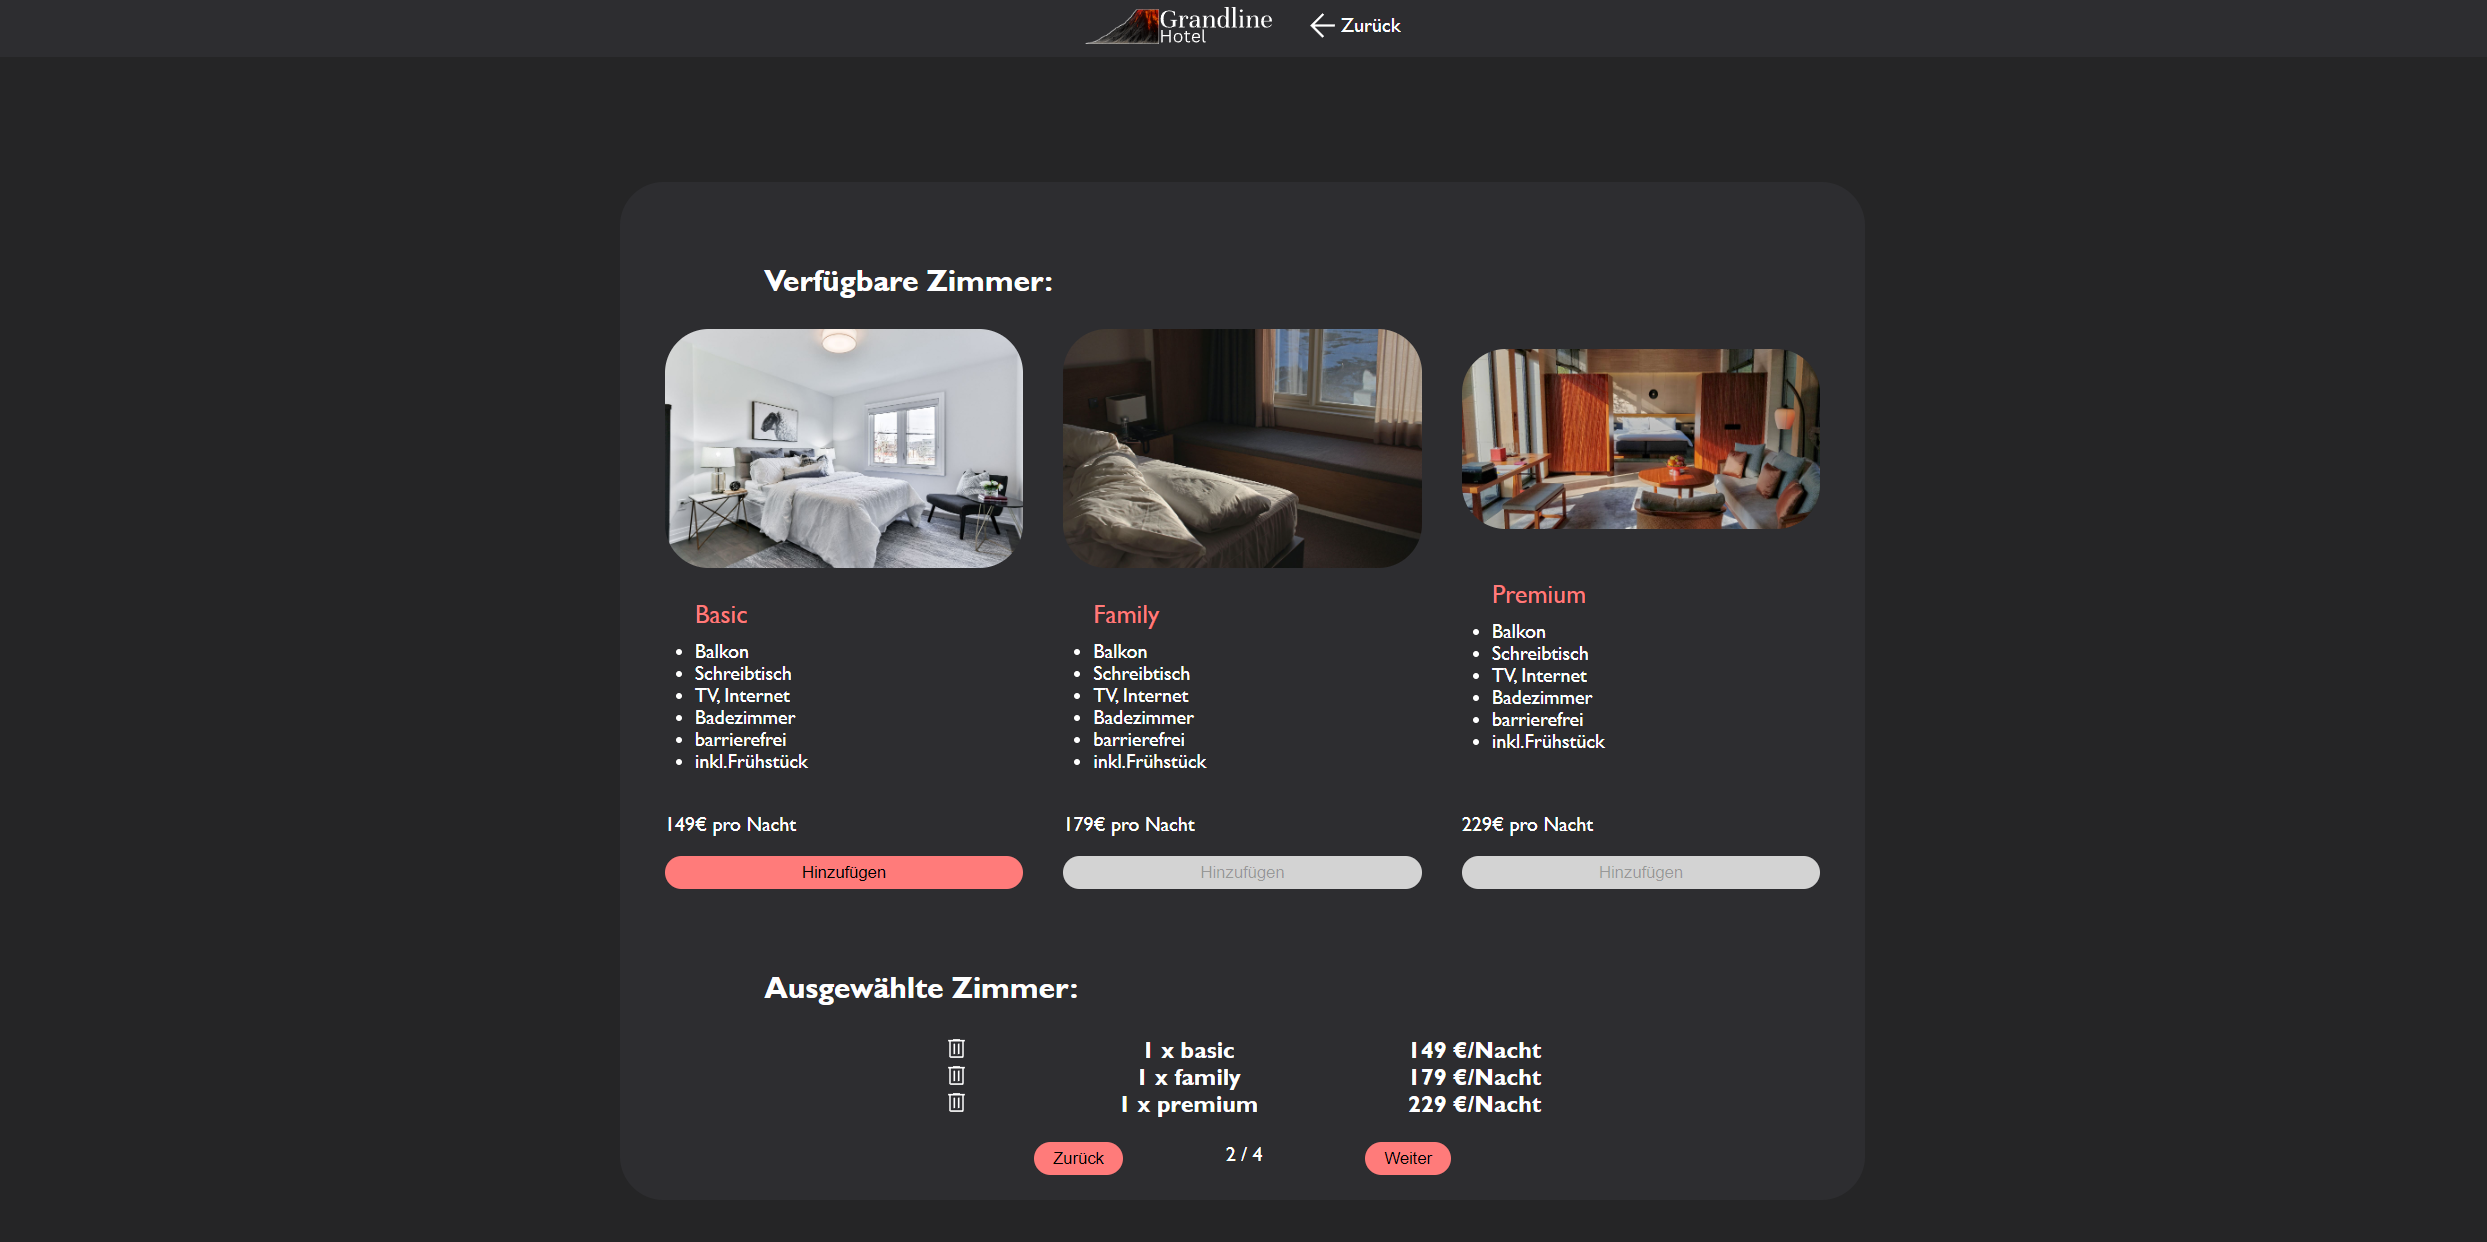
\includegraphics[width=\textwidth]{images/Beispiel/Schritt5.png}
	\caption{Schritt 5}
	\label{step5}
\end{figure}
\newpage
In das nun erschienene Formular trägt der Nutzer seine persönlichen Daten ein und fährt über den \glqq Weiter\grqq-Knopf mit dem Buchungsdialog fort (siehe Abb.\ref{step6}).
\begin{figure}
	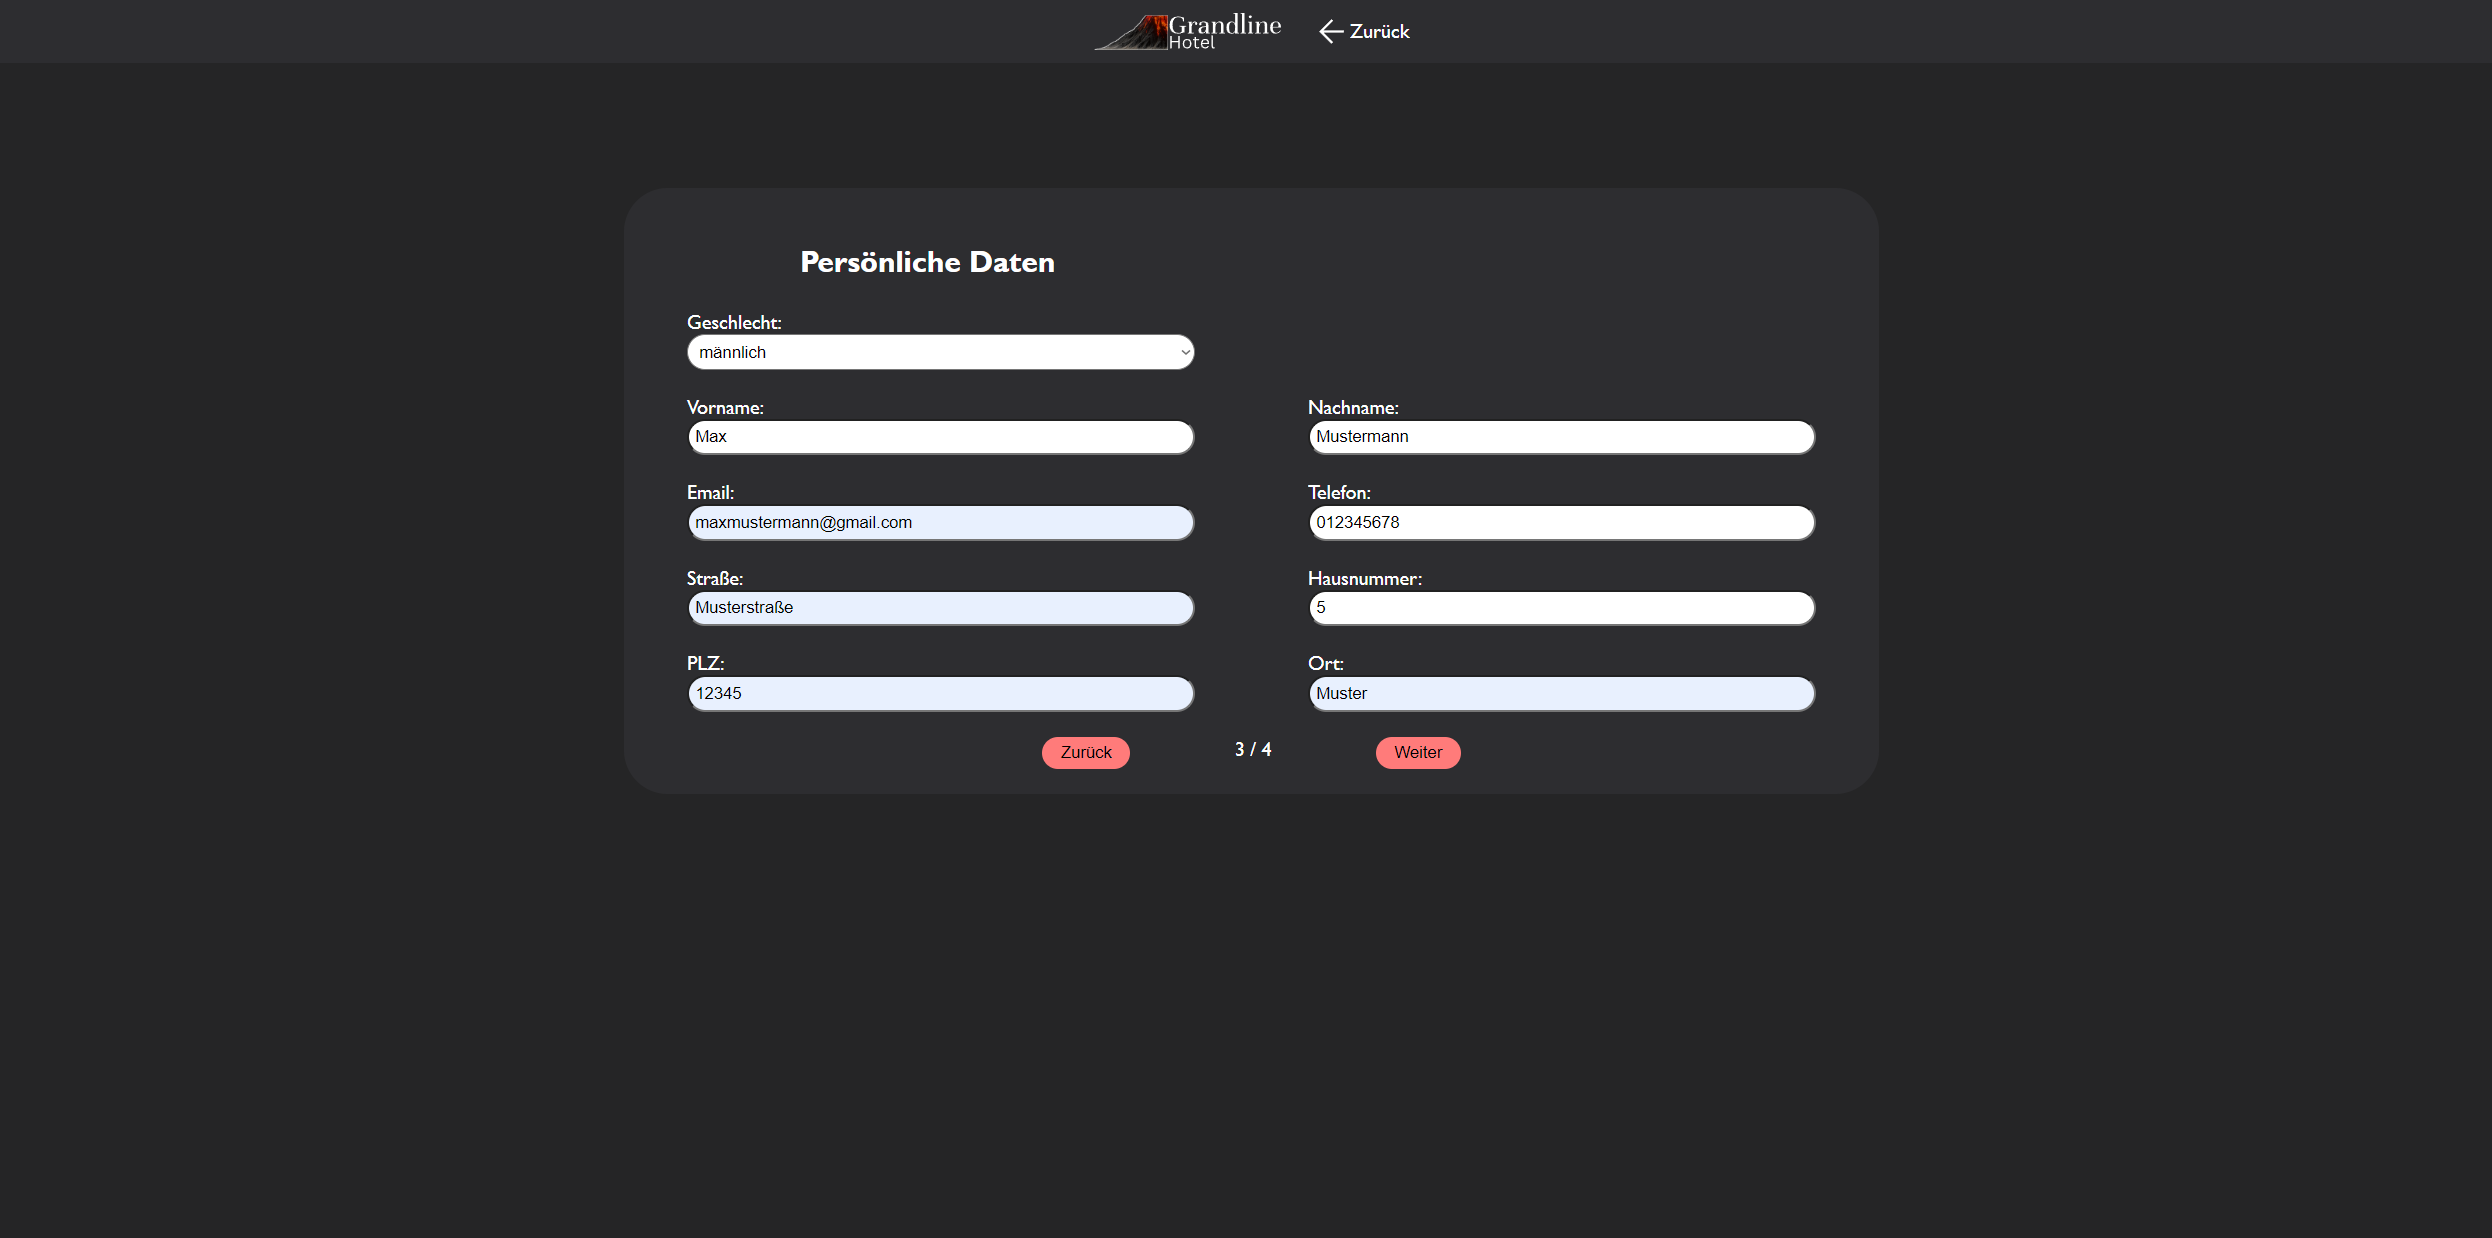
\includegraphics[width=\textwidth]{images/Beispiel/Schritt6.png}
	\caption{Schritt 6}
	\label{step6}
\end{figure}
\newline
Im siebten Schritt wird dem Nutzer eine Übersicht über die zu tätigende Buchung dargeboten und bietet dem Nutzer vor dem Abschluss die Möglichkeit noch Extrawünsche und Informationen über ein Textfeld an das Hotel weiterzugeben (siehe Abb.\ref{step7}). Klickt der Nutzer anschließend auf \glqq Abschließen\grqq, wird der Buchungsprozess abgeschlossen.
\begin{figure}
	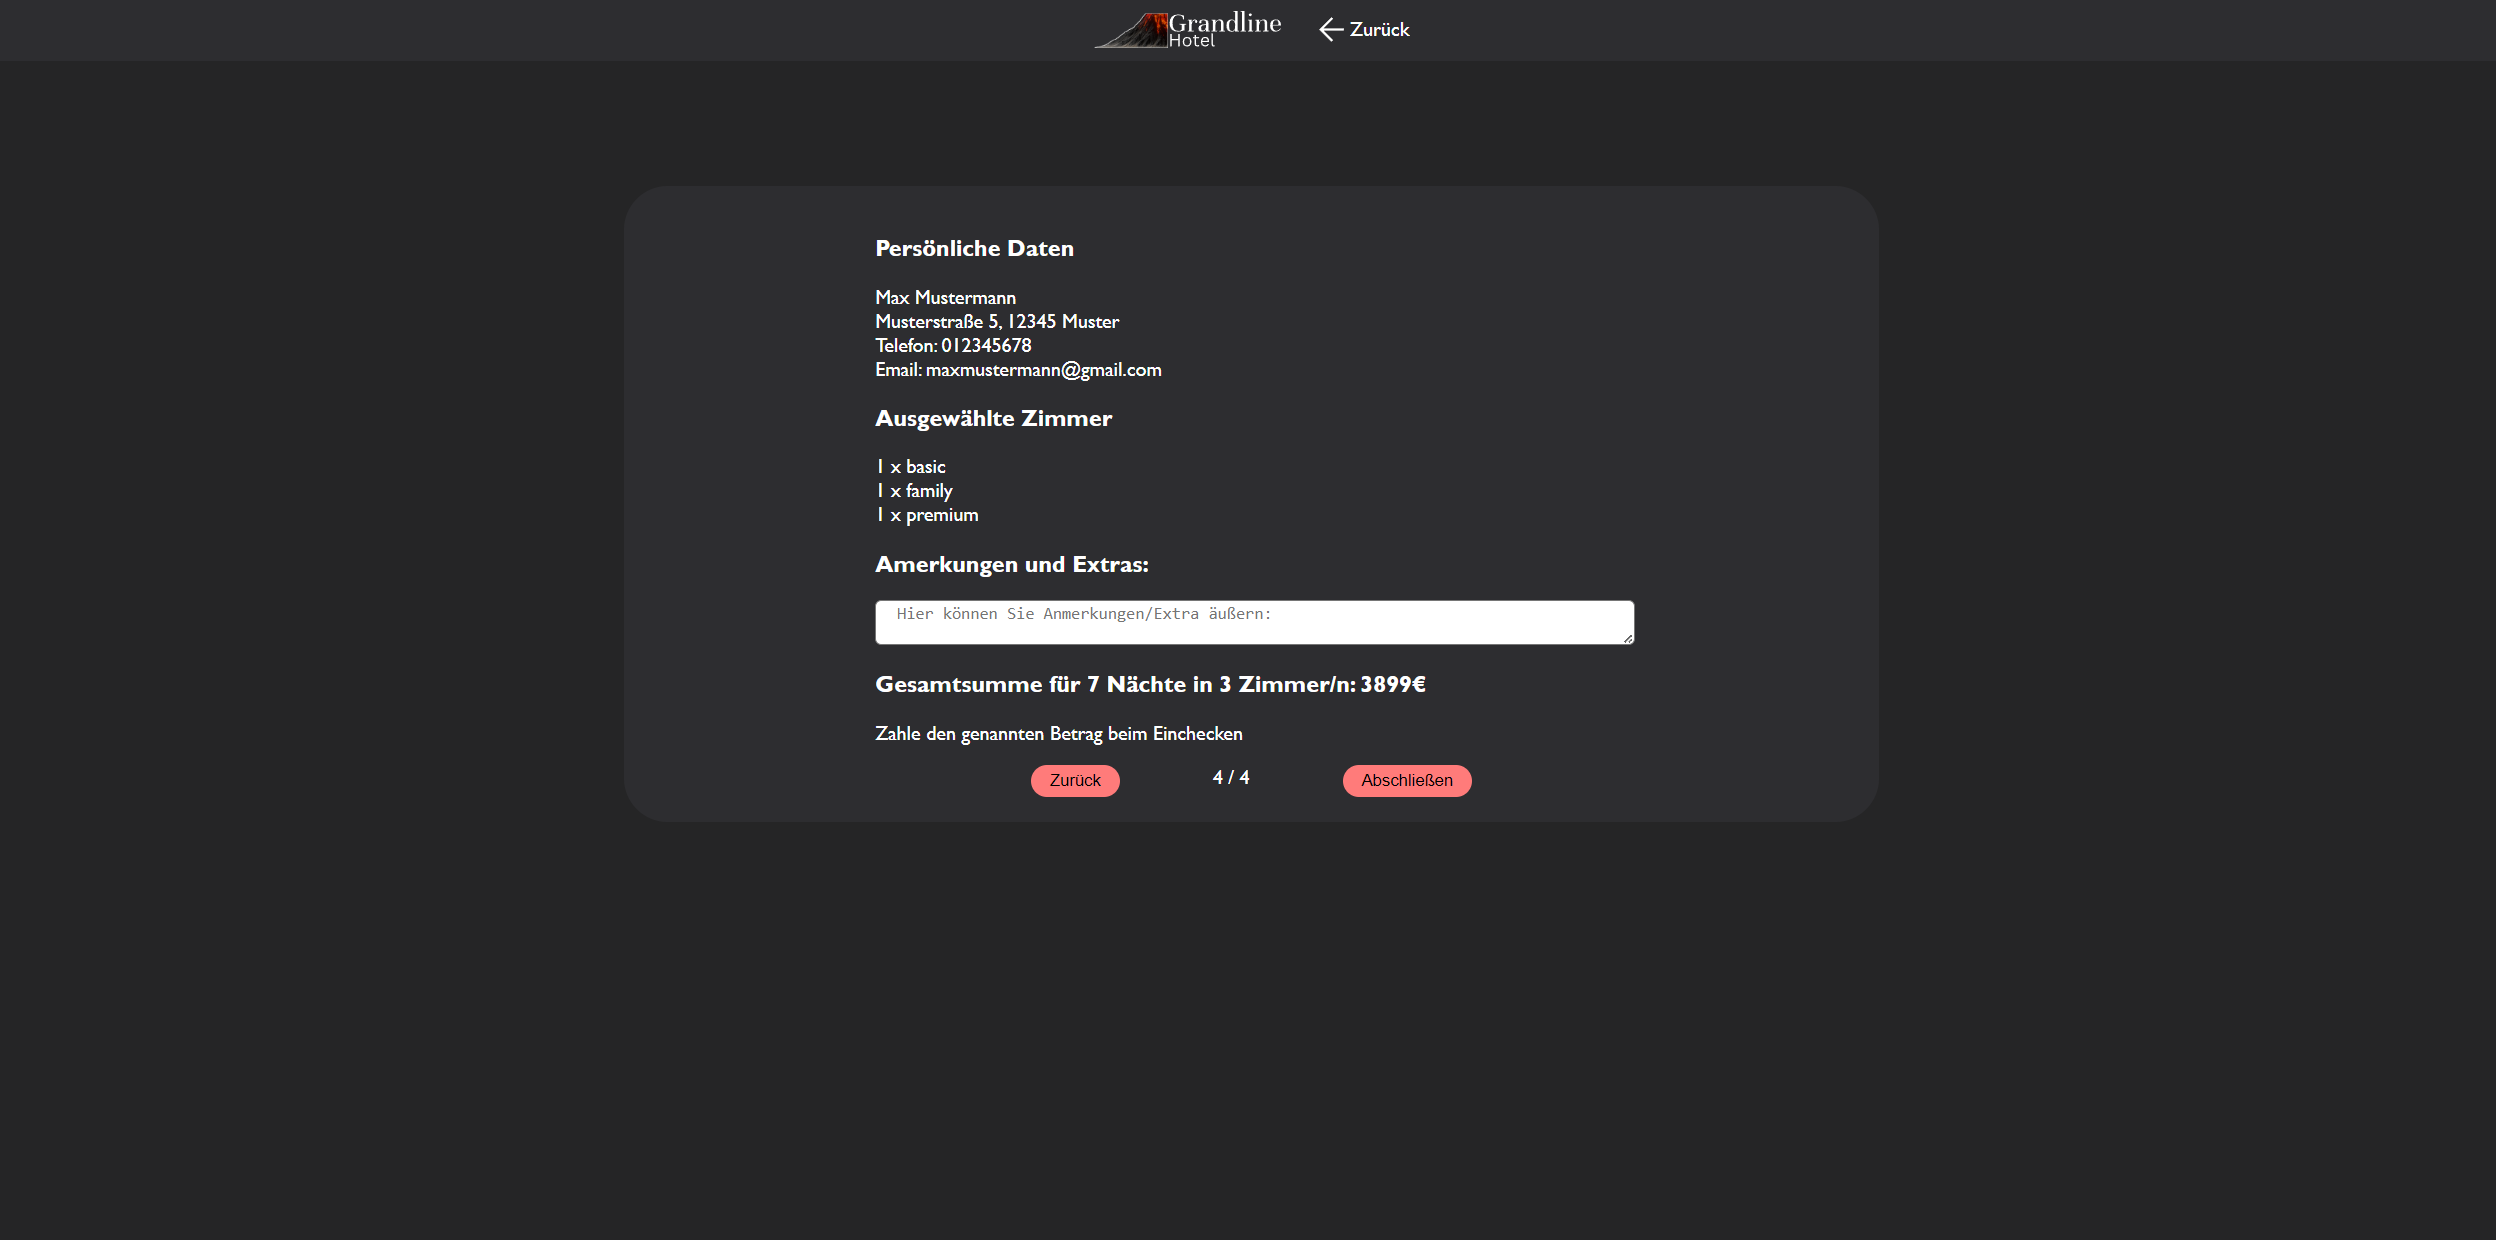
\includegraphics[width=\textwidth]{images/Beispiel/Schritt7.png}
	\caption{Schritt 7}
	\label{step7}
\end{figure}
\newpage
Nach Abschluss der Buchung wird der Nutzer darüber informiert, dass eine E-Mail mit den wichtigsten Informationen an den Nutzer versendet wurde (siehe Abb.\ref{step8}).
\begin{figure}
	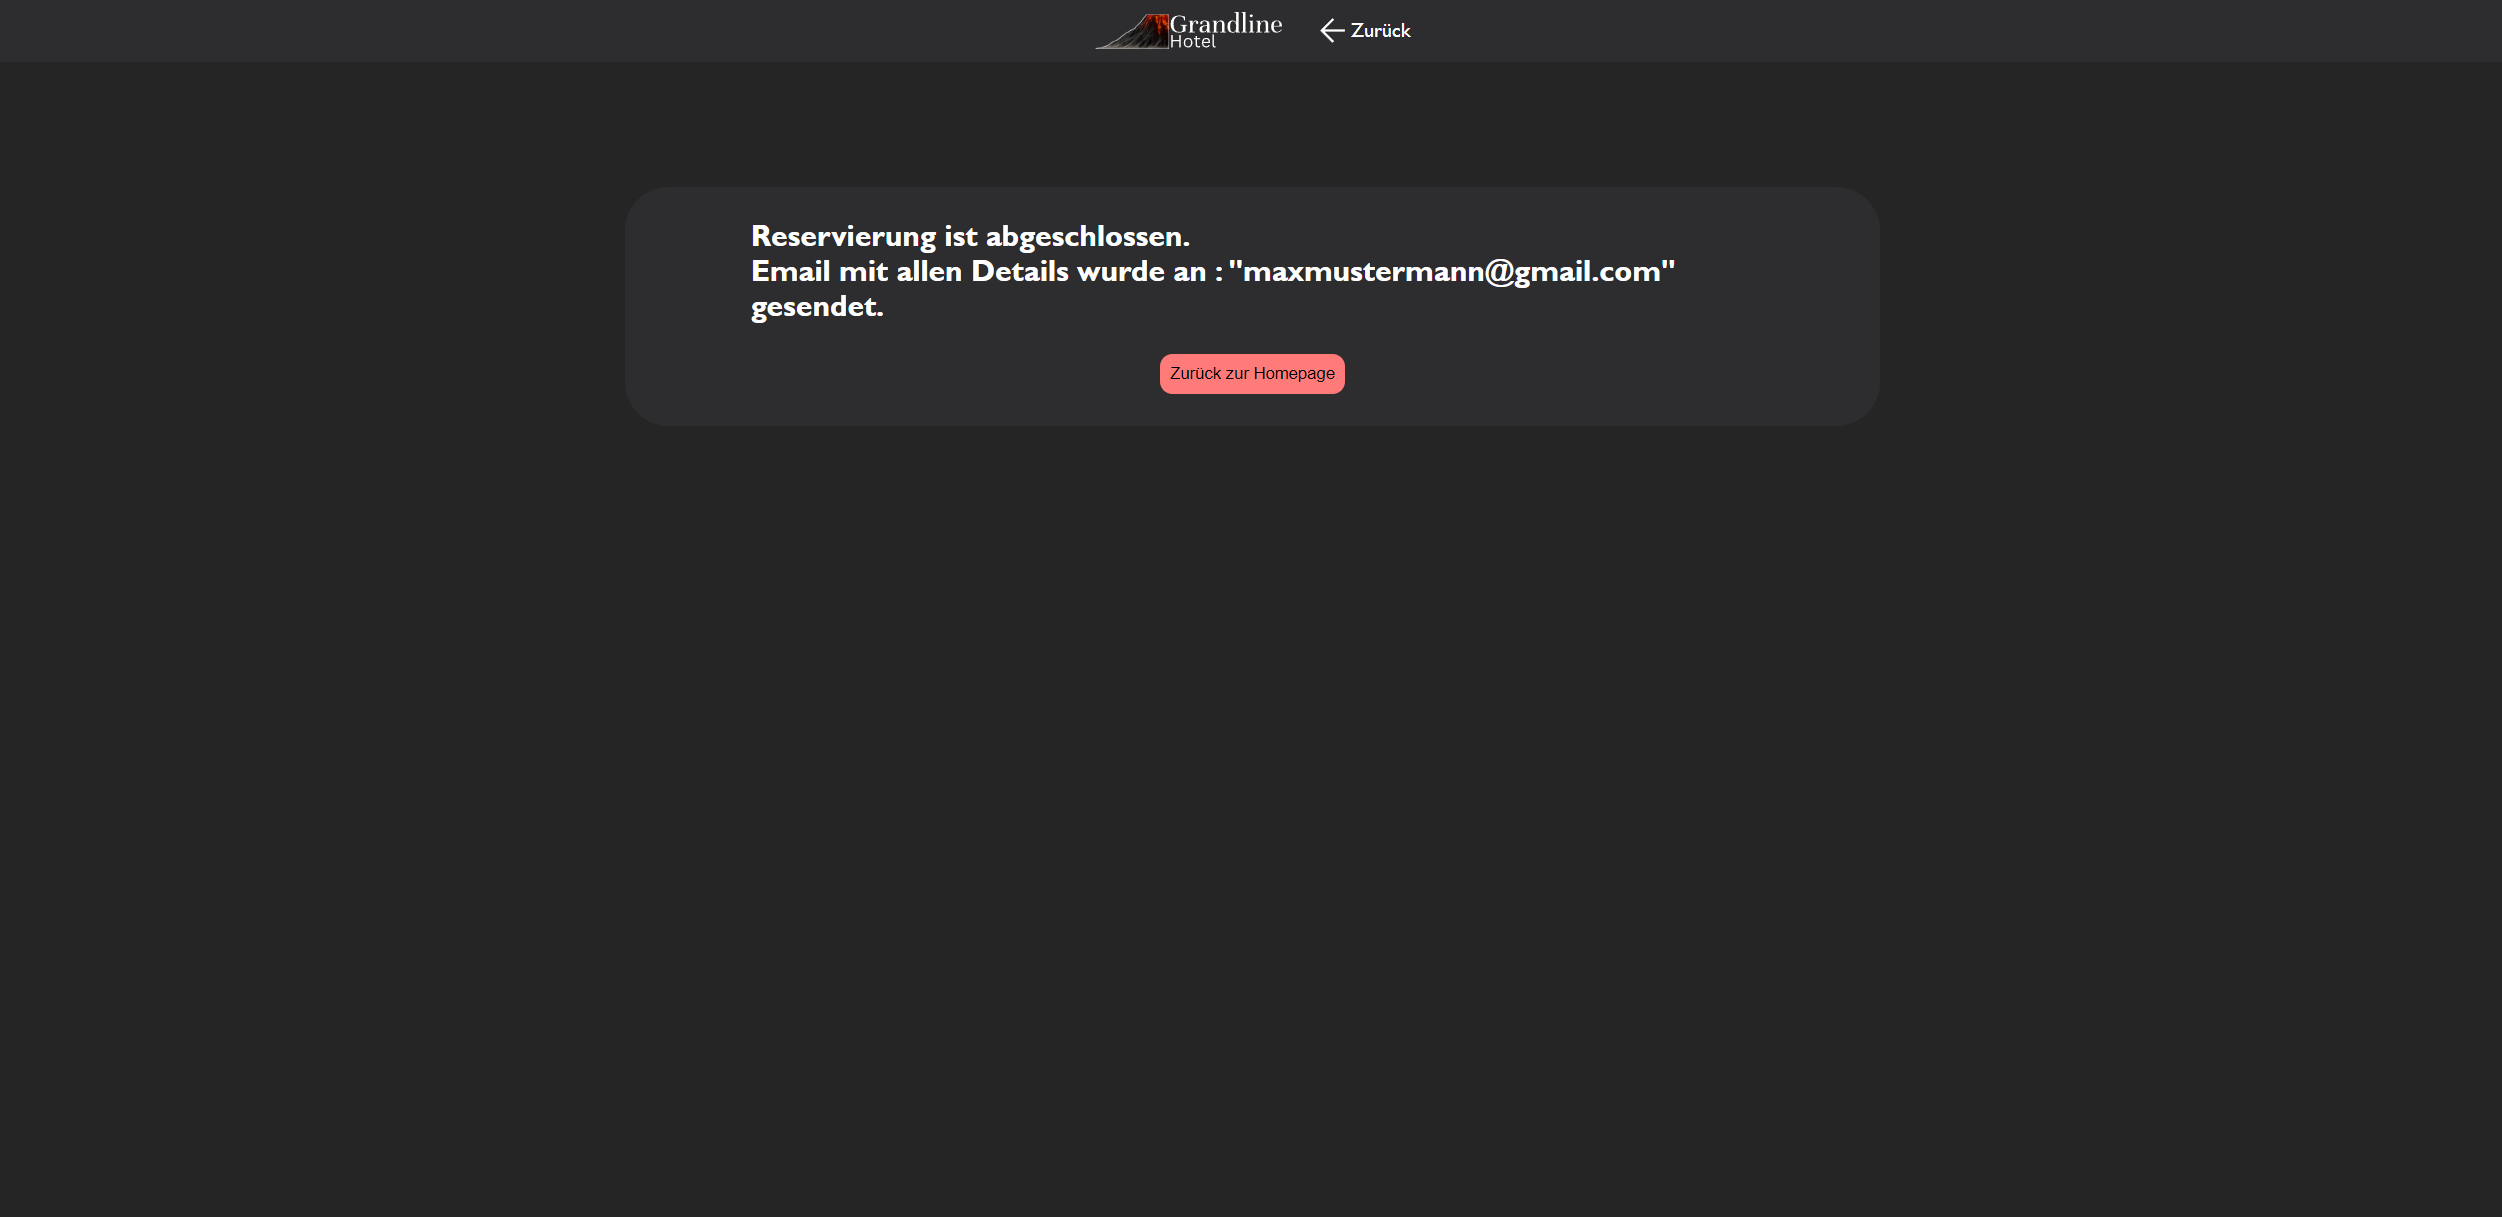
\includegraphics[width=\textwidth]{images/Beispiel/Schritt8.png}
	\caption{Schritt 8}
	\label{step8}
\end{figure}